$if(has-frontmatter)$
\frontmatter
$endif$

% ===========================================================================
%  PORTADA
% ===========================================================================
\begin{titlepage}
\thispagestyle{empty}
\begin{tikzpicture}[remember picture, overlay]

  % Reproduce assets/portada.svg (lienzo de 800 x 1132 unidades). Las
  % posiciones se dan en unidades del SVG, escaladas al tamaño del papel,
  % y se miden desde la esquina superior izquierda de la página.
  \pgfmathsetlengthmacro{\ux}{\paperwidth/800}
  \pgfmathsetlengthmacro{\uy}{\paperheight/1132}
  \pgfmathsetlengthmacro{\anchoilustracion}{541.2*\ux}
  \pgfmathsetlengthmacro{\altoilustracion}{529.6*\uy}

  % Fondo
  \fill[eaVerdeOscuro] (current page.north west) rectangle (current page.south east);

  % Trama de puntos en la mitad superior
  \foreach \x in {0,...,19}{
    \foreach \y in {0,...,13}{
      \fill[white, opacity=0.08]
        ([xshift=10*\ux+\x*40*\ux, yshift=-10*\uy-\y*40*\uy]current page.north west)
        circle (3*\ux);
    }
  }

  % Ilustración: captura de la aplicación
  \node[anchor=north west, inner sep=0pt]
    at ([xshift=129.4*\ux, yshift=-75.4*\uy]current page.north west)
    {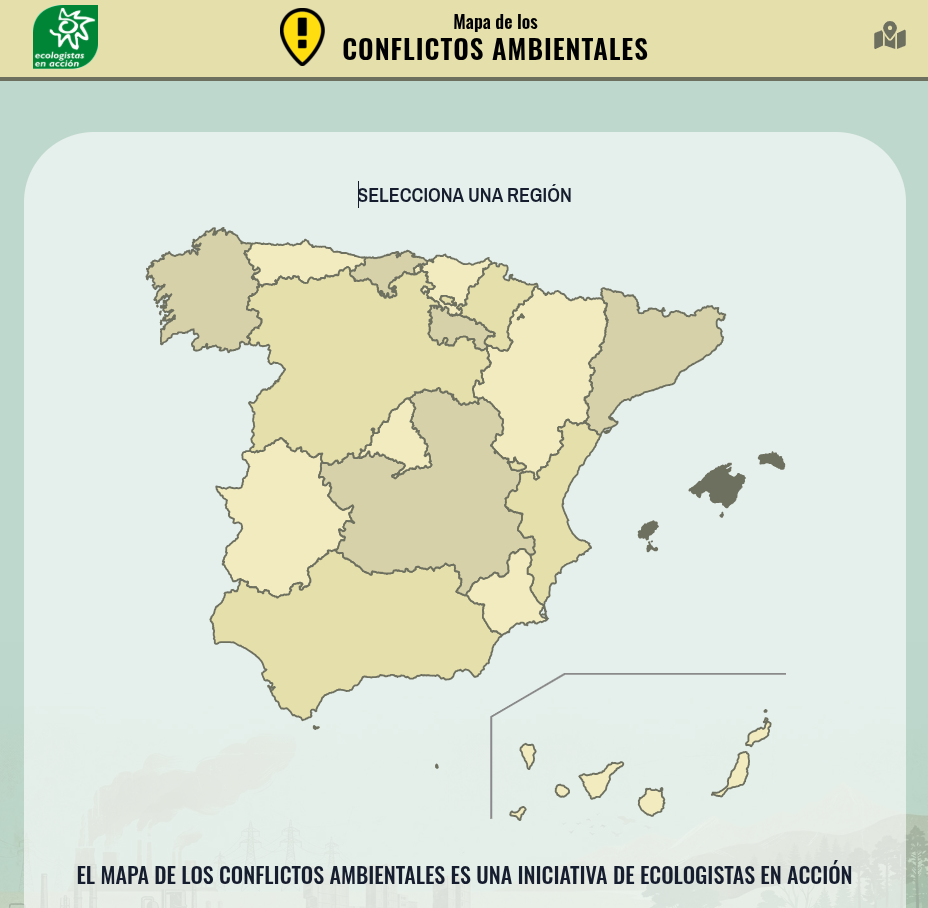
\includegraphics[width=\anchoilustracion, height=\altoilustracion]{assets/portada-ilustracion.png}};

  % Título en tres líneas, como en la portada SVG
  \foreach \linea/\base in {Mapa de/710, Conflictos/782, Ambientales/854}{
    \node[anchor=base west, inner sep=0pt]
      at ([xshift=90*\ux, yshift=-\base*\uy]current page.north west)
      {\color{white}\sffamily\bfseries\fontsize{48}{51}\selectfont \linea};
  }

  % Filete
  \fill[white]
    ([xshift=90*\ux, yshift=-890*\uy]current page.north west) rectangle
    ([xshift=270*\ux, yshift=-895*\uy]current page.north west);

$if(subtitle)$
  % Subtítulo
  \node[anchor=base west, inner sep=0pt]
    at ([xshift=90*\ux, yshift=-945*\uy]current page.north west)
    {\color{eaNaranjaClaro}\sffamily\fontsize{22}{26}\selectfont $subtitle$};
$endif$

  % Entidad editora
  \node[anchor=base west, inner sep=0pt]
    at ([xshift=90*\ux, yshift=-1045*\uy]current page.north west)
    {\color{white}\sffamily\fontsize{16}{19}\selectfont Ecologistas en Acción};

  % Franja inferior
  \fill[eaNaranja] (current page.south west) rectangle
    ([yshift=24*\uy]current page.south east);

\end{tikzpicture}
\end{titlepage}

% ===========================================================================
%  PÁGINA DE CRÉDITOS
% ===========================================================================
\thispagestyle{empty}
\null\vfill
\noindent
{\sffamily\bfseries\large\color{eaVerdeOscuro} $title$}\\[0.2em]
$if(subtitle)$
{\sffamily\color{eaGris} $subtitle$}\\[1.2em]
$endif$
{\footnotesize\sffamily\color{eaGris}
\noindent Aplicación web: \url{https://conflictosambientales.ecologistasenaccion.org/}\\[0.4em]
\noindent Edita: Ecologistas en Acción\\[0.4em]
\noindent Esta obra se distribuye bajo licencia Creative Commons
Reconocimiento-CompartirIgual 4.0 Internacional (CC BY-SA 4.0).\\[0.4em]
\noindent Versión del manual: 0.1 (borrador). Las capturas de pantalla pueden
no corresponder con la última versión de la aplicación.\par}
\vspace{1.5cm}
\clearpage

$if(abstract)$
\begin{abstract}
$abstract$
\end{abstract}
$endif$
